\section{Survey data in American households}\label{section:surveyData}
%What is the NHIS, is it good, reputable etc? Show other studies linked to this data source
\subsection{The National Health Interview Survey}
The data used in this application is obtained from the National Health Interview Survey (NHIS) \citep{NHIS-original}, with an extract taken from the publicly available IPUMS NHIS database \citep{IPUMS}, accessible at \url{https://nhis.ipums.org/}. The NHIS is a public ongoing cross-sectional household survey of health in the United States where participants have been sampled every month since $1957$ using geographically clustered sampling techniques. Every month, the newly collected sample is designed to be nationally representative of the civilian, non-institutionalized population, with annual samples of households between 30,000 and 50,000, covering about 75,000 to 100,000 participants. The participants are surveyed to collect information on topics such as general health, living conditions, and health behaviors (exercise, diet, alcohol consumption etc.). The survey data aids researchers in examining the distribution of health conditions by characteristics such as demographic or socioeconomic factors, which allows them to answer their research questions. For the application in this thesis, we will be looking at the health outcome of back pain stratified by level of education.

%how do they aquire their data, what do they have available
The NHIS is a household study, meaning that households are sampled at the top level of the sampling hierarchy. Each household may contain one or several families, where one representative from each family provides information on the demographic and health related status for each family member. In addition to the data collected from each family member, one child and one adult from each family are sampled and interviewed in greater detail. Through this additional interview, the NHIS collects further information on the Body Mass Index, mental health, physical health, access to health care, and personal health behaviors. The adult participants are also interviewed about information pertaining to their employment and education. This data is released annually in standalone data sets for several levels of the sampling hierarchy.

%What data do use specifically
Although data is available from $1957$ to the present day, we focus our attention in this thesis to the data collected between and including $1997$ and $2018$, as the general survey design was largely unchanged during this period. A few minor changes were made to the collection design, sampling strategy and questions, making the survey results from each year comparable, and resulting in suitable data for temporal analyses. Our data extract uses the data available at the adult level, containing 580,072 samples from individuals aged $25$ to $84$. Each collected sample, along with the level of attained education, contains the recorded presence or absence of back pain in the year and month of observation. The attained education levels are grouped into $4$ categories; less than high school/general
educational development (LHS/GED), high school (HS), some college or associate of arts degree (SC/AA), and bachelor degree or higher (BA+). Moreover, demographic data is available for each participant, such as sex, race, age, and whether the participant was born in a country other than the United States. The raw data extract is available on an individual-specific level, though (for our models) it is more sensible to aggregate the data. In this case, the data will be aggregated by year, age, and education. In the case of back pain, we simply summarize the number of participants with present back pain and the total number of participants in the specified group. Further specifications on how the data is aggregated and used are provided in Section \ref{section:application1:specification}.

%Survey design issues
The sampling scheme of the NHIS is quite complex for several reasons, most notably due to the multistage sampling, clustering techniques, and dynamic sampling strategy of minority populations. The NHIS divides the United States into $1,689$ pseudo sampling units (PSUs), typically counties or groups of counties, which are then grouped into different strata based on social and demographic characteristics. Every year in the design period of $1997$ to $2015$, one or more PSUs were sampled for each stratum based on the within-stratum population size of the PSUs. Geographic areas were then sampled within each PSU and divided into small clusters of housing units, which were then surveyed randomly. From 2016 and onwards, the PSUs are divided into one or two strata, depending on the urbanity of the PSU, after which clusters of approximately 2,500 addresses are identified within each stratum, in which some number of the addresses are sampled. In addition to this, race and ethnic groups were strategically oversampled in varying timeframes in the design period of $1997$ to $2018$ (Blacks; $1985$ to $2015$, Hispanics; $1995$ to$2015$, and Asians; $2006$ to $2015$). These sampling strategies and techniques are typically accounted for by use of the PSU and stratum indicators, along with post-stratification weights provided by the survey. 

\subsection{Explorative analysis of back pain data for males and females}
\label{section:data:explorative}
In anticipation of the upcoming analysis of the survey data using the Bayesian multivariate APC model (to be introduced), exploratory analysis of the obtained NHIS survey data is carried out to supply context to later analysis. As will be shown in Section \ref{section:APC-inference}, the inference provided by the multivariate APC model revolves around differences in the effects attributed to the age, period, and cohort with respect to a specified level of education. That is, the inference is relative to the rate of back pain in the chosen baseline level of education. Therefore, to make sense of the inference in the upcoming multivariate APC analysis, simple exploratory analysis is carried out by examining the data empirically over the age, period, and cohort groups of the data stratified by level of education. As we will be considering multivariate APC models in later analysis separately by sex, the exploratory analysis is carried out separately for males and females.

Side by side for females and males, Figure \ref{figure:data_numb} shows the total number of participants stratified by level of education in each age group, period, and birth cohort. Over age, younger adults are generally sampled more frequently than older adults in all levels of attained education. In the two lowest levels of attained education, LHS/GED and HS, a large difference in the number of participants is observed for younger adults compared to the two other levels of attained education, though this difference is smaller in older age groups, particularly in males. Over periods, in both females and males with LHS/GED level of attained education, significantly fewer samples are collected compared to the three other levels. Among the participants of both sexes with HS, SC/AA, and BA+ levels of attained education, we observe similar sample sizes in earlier periods, though after $2006$, the differences in the sample sizes based on level of attained education becomes clearer. In older cohorts, greater sample sizes in the LHS/GED and HS levels of attained education are observed compared to SC/AA and BA+, though this is reversed by the $1940$ birth cohort. Taken together, in terms of sample sizes, it appears that the population with BA+ level of attained education is best represented over all temporal indices, while the population with LHS/GED level of attained education is the worst represented. 

\begin{figure}[!ht]
    \begin{minipage}{.8\textwidth}
    \centering
    \begin{subfigure}[b]{\textwidth}   
        \centering 
        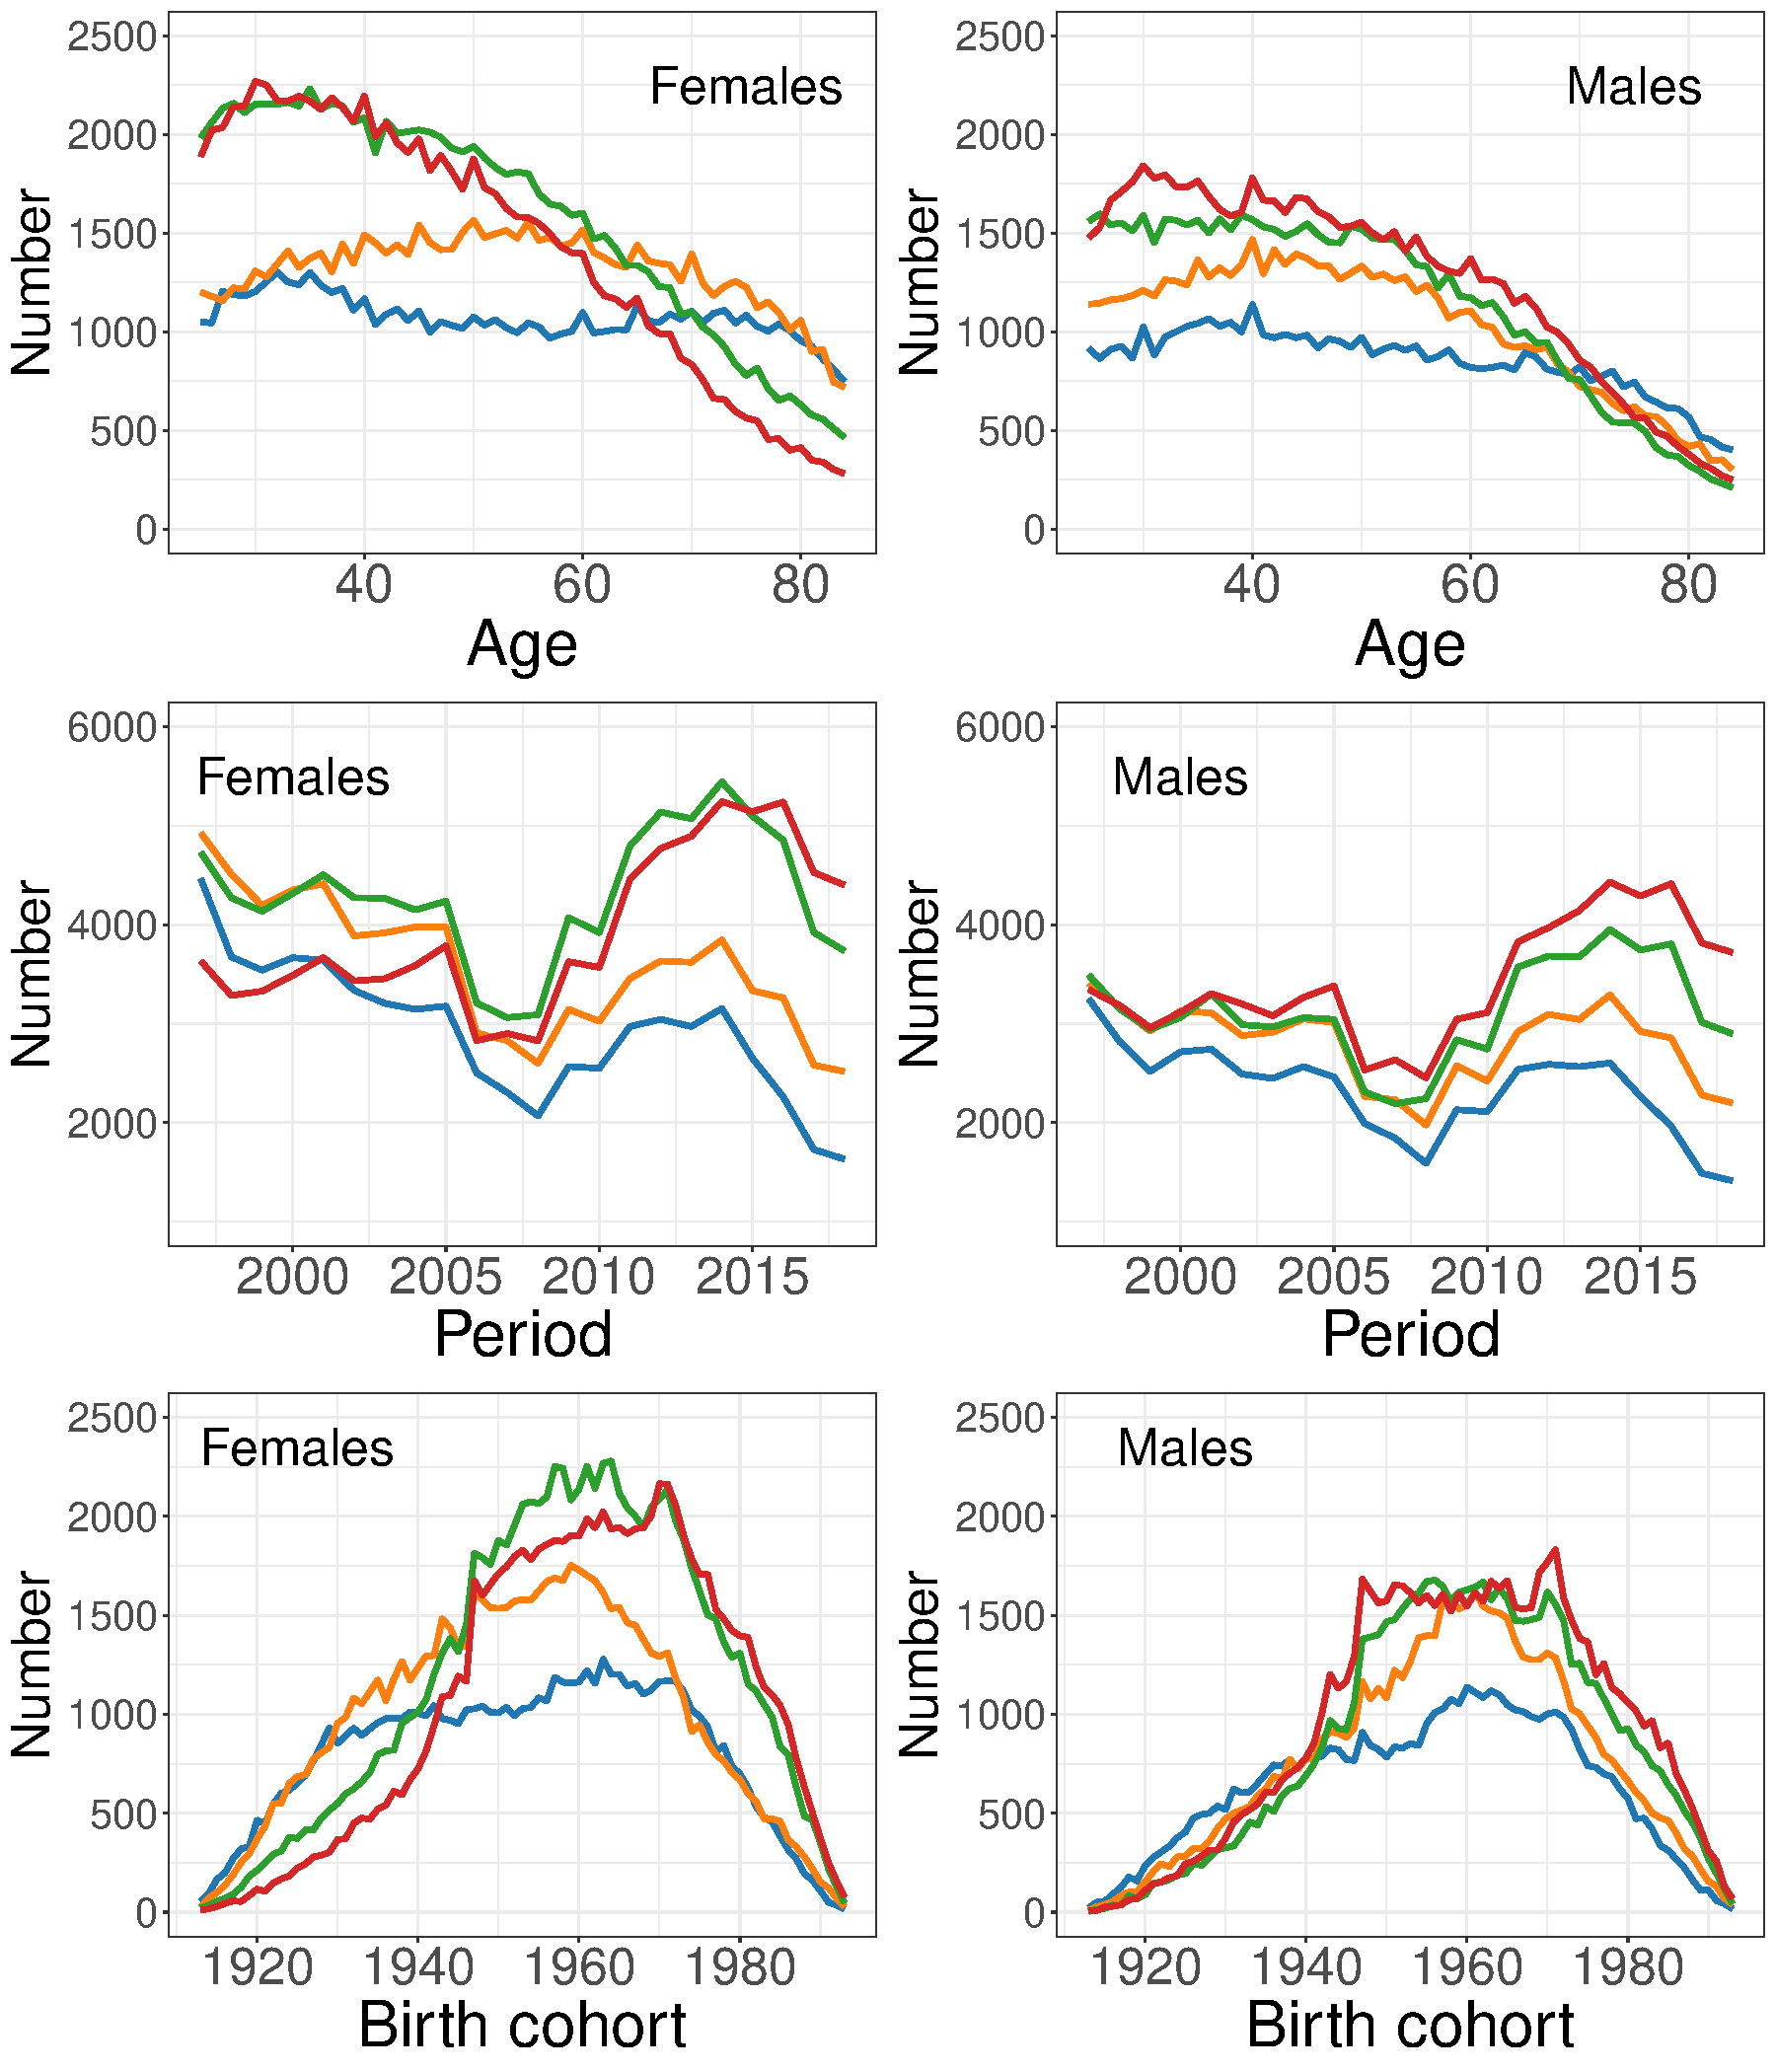
\includegraphics[width=\textwidth]{Figures/numbers.pdf}
    \end{subfigure}
    \vskip\baselineskip\vspace{-0.3cm}
    \end{minipage}%
    \begin{minipage}{.2\textwidth}
        \hfill\vspace{-1.0cm}
        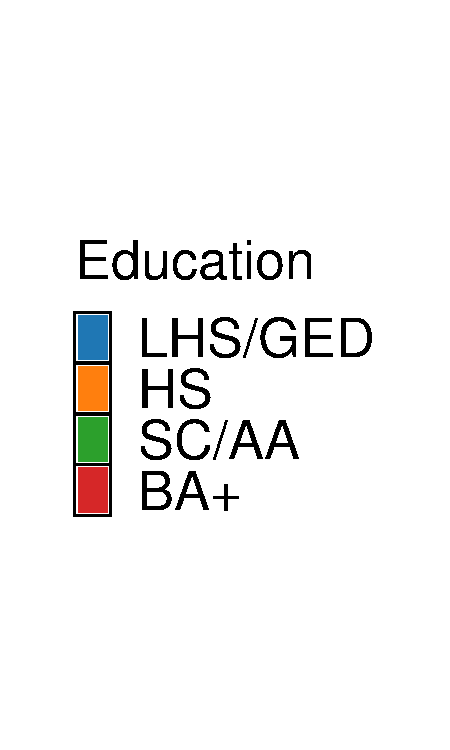
\includegraphics[width = \textwidth]{Figures/number_prop_legend_m.pdf}
    \end{minipage}
    \caption{The number of (left) female and (right) male participants in the survey data grouped by age group, period, and birth cohort, separated by level of attained education.}
    \label{figure:data_numb}
\end{figure}

\begin{figure}[!ht]
  \begin{minipage}{.8\textwidth}
  \centering
  \begin{subfigure}[b]{\textwidth}   
      \centering 
      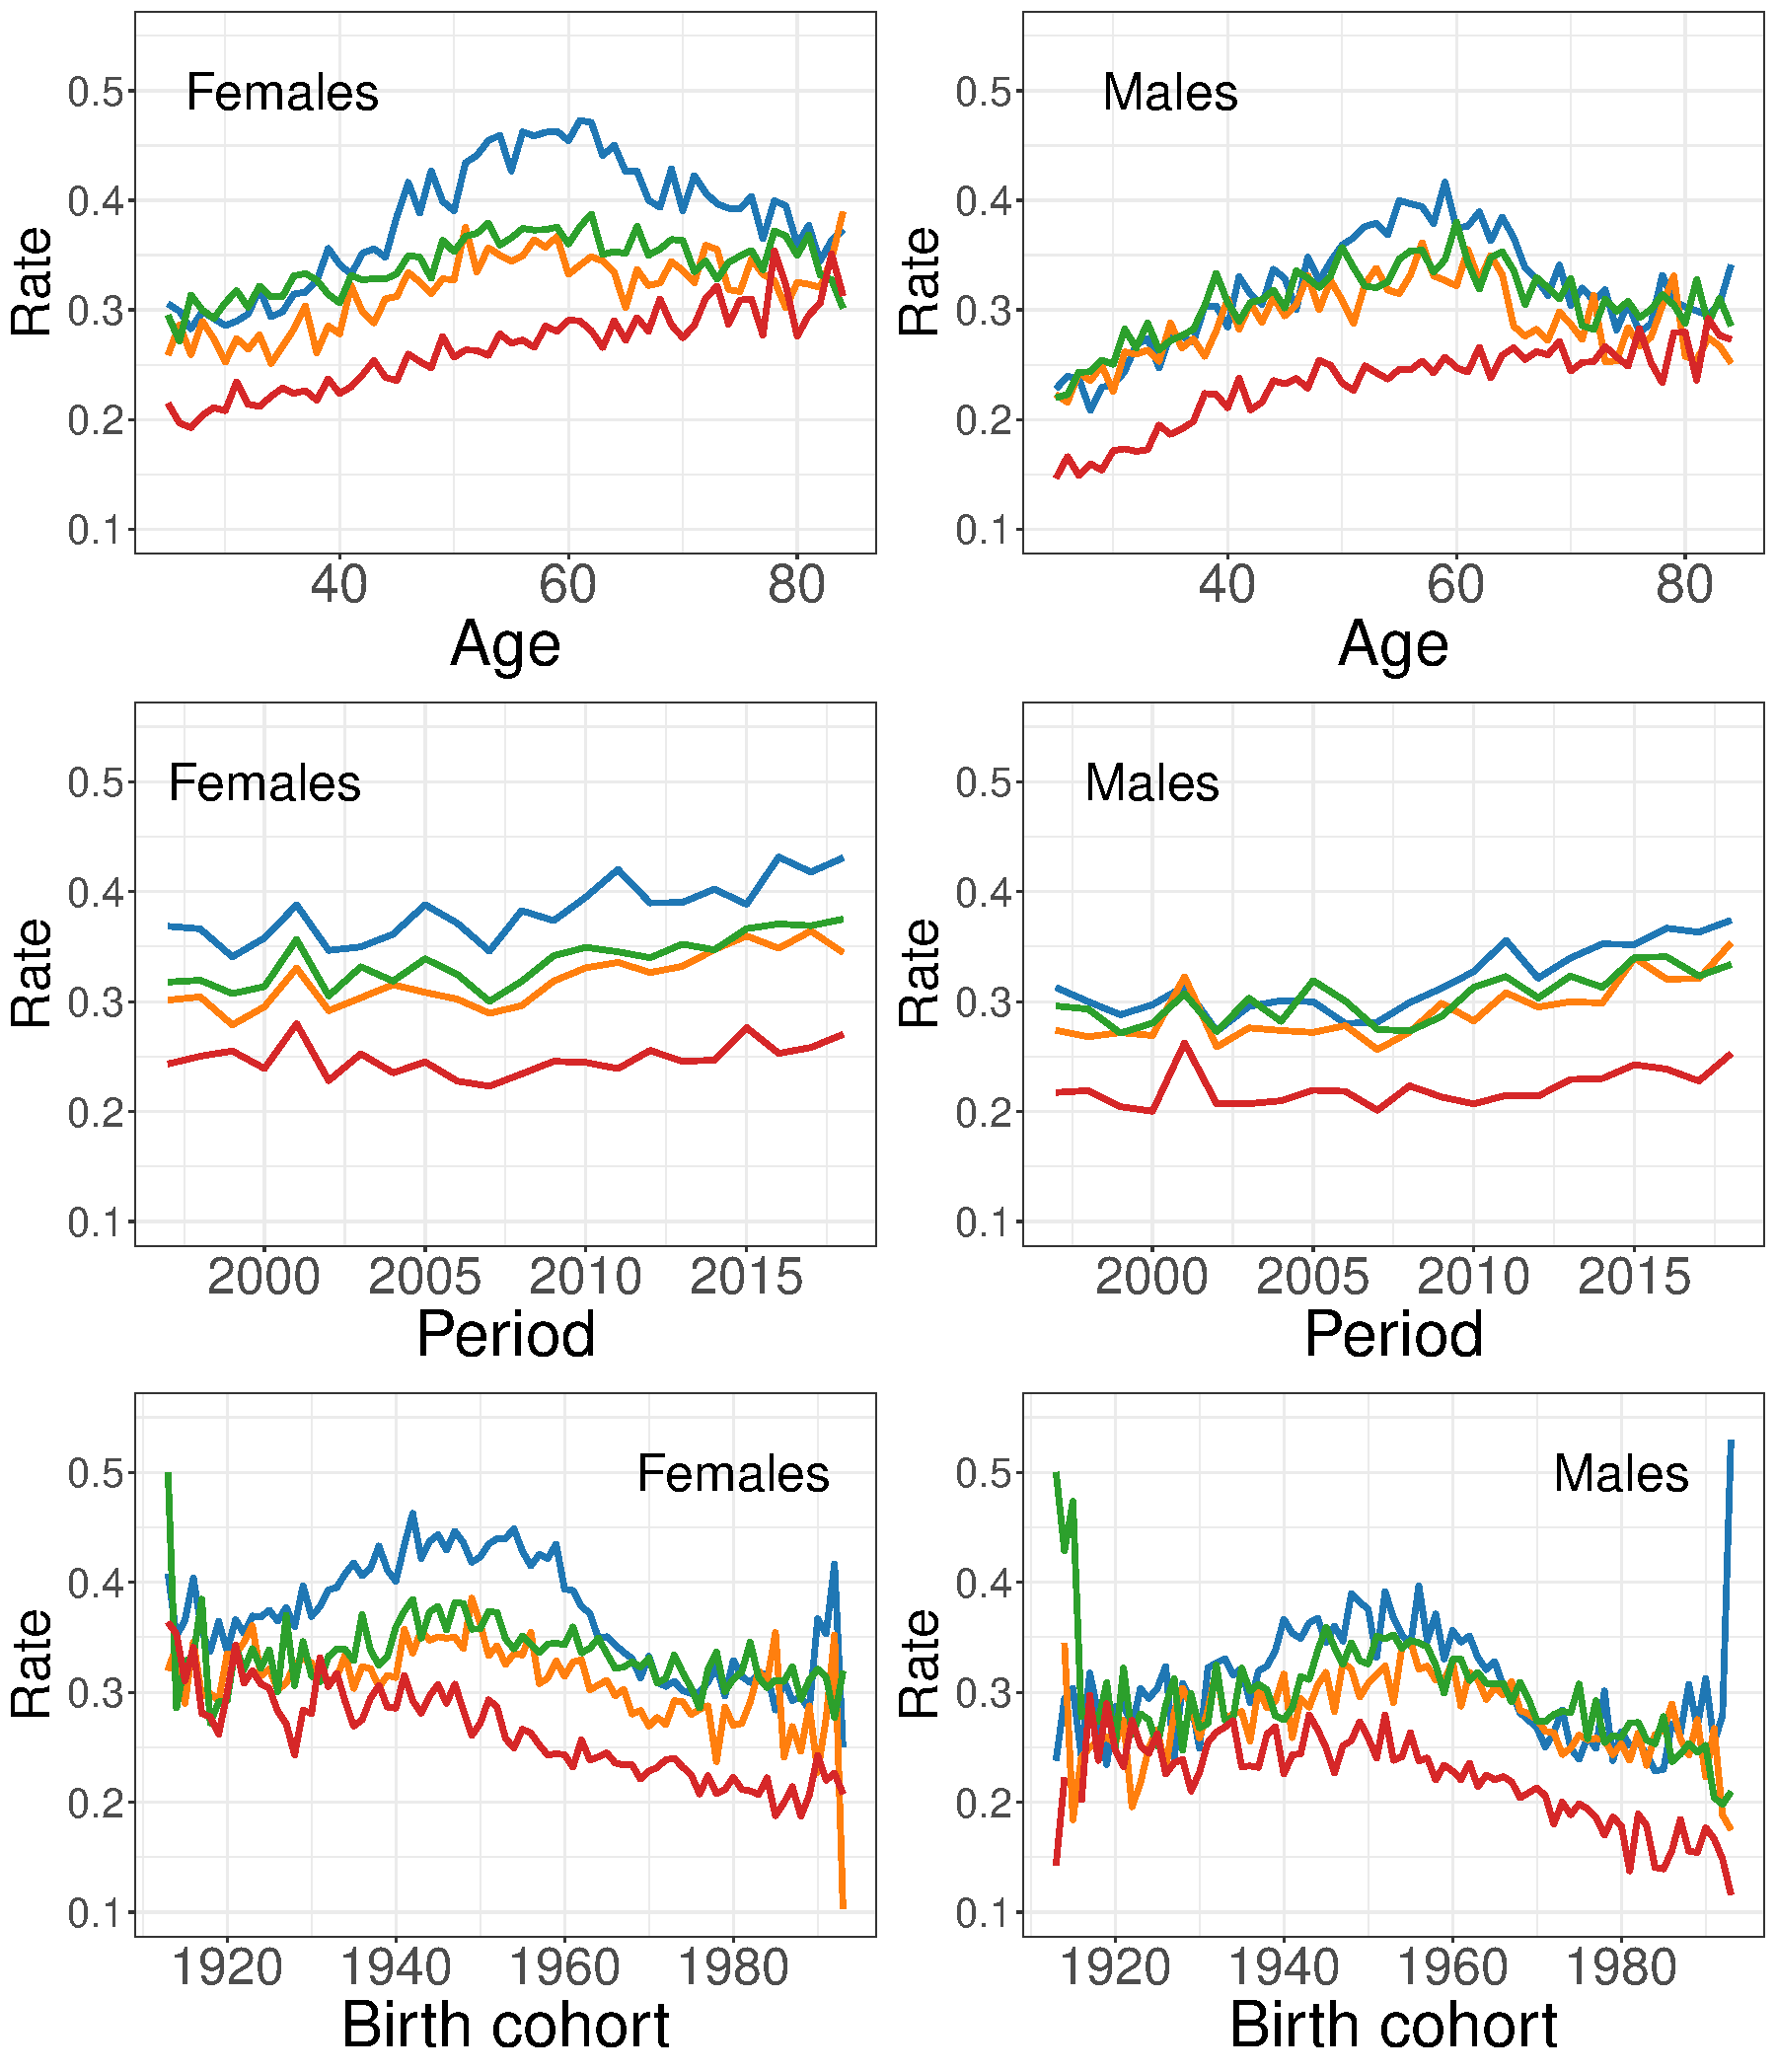
\includegraphics[width=\textwidth]{Figures/proportions.pdf}
  \end{subfigure}
  \vskip\baselineskip\vspace{-0.3cm}
  \end{minipage}%
  \begin{minipage}{.2\textwidth}
      \hfill\vspace{-1.0cm}
      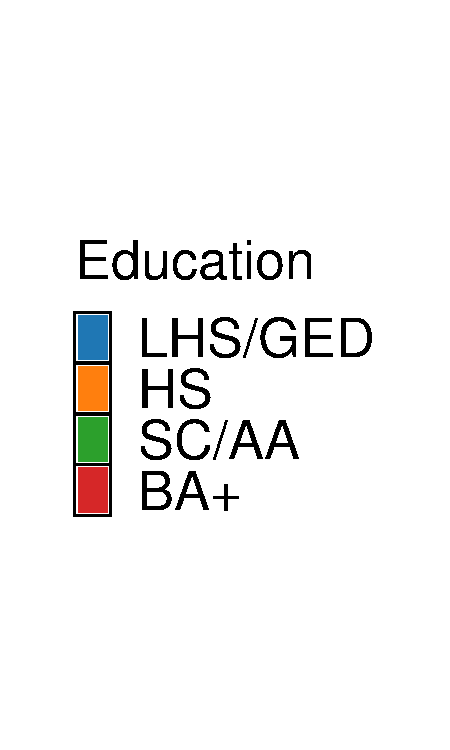
\includegraphics[width = \textwidth]{Figures/number_prop_legend_m.pdf}
  \end{minipage}
  \caption{The proportion of (left) female and (right) male participants with back pain in the survey data grouped by age group, period, and birth cohort, separated by level of attained education.}
  \label{figure:data_prop}
\end{figure}

The proportion of participants reporting back pain, stratified by level of education in each age group, period and birth cohort is shown in Figure \ref{figure:data_prop}, side by side for females and males. In both females and males, over age, the proportions appears to be generally increasing until age $60$ after which it decreases among participants with LHS/GED level of attained education, while remaining almost constant for the others. Over periods, the proportions appears to be nearly constant or slightly increasing for both females and males in all levels of attained education. Over cohorts, the proportions are either slightly increasing or constant between the $1913$ and $1950$ birth cohorts. In more recent cohorts after the $1950$ birth cohort, the proportions appear to decrease for all levels of attained education. Across all three temporal indices, it is evident that participants with BA+ level of attained education generally experienced back pain more seldom than the lower levels of attained education. Conversely, participants with the lowest level of education, LHS/GED, appears to generally have experienced the highest proportions of back pain over all three temporal indices. For the two other levels of attained education, HS and SC/AA, their proportions of individuals with back pain generally appear to be closer to that of LHS/GED than BA+. 

Figures \ref{figure:explorative:rateplot_age_f} and \ref{figure:explorative:rateplot_age_m} show the rate of back pain over the years of observation in survey participants grouped by age for females and males, respectively. Within all age groups, for all levels of attained education, the rate appears to be either slightly increasing or constant, albeit with some fluctuation. Across levels of education, we observe different rates, with the highest-observed rate for LHS/GED level ($25\%$ to $50\%$), and the lowest-observed rate for BA+ level ($19\%$ to $35\%$). For HS and SC/AA levels of attained education, the rate appears to be similar over periods. Interestingly, among participants with GED/LHS level of attained education, the rate between age groups differs the most compared to all other levels of attained education. In both figures, as we advance through the age groups from youngest to oldest, we observe, for all levels of attained education, increasing rate until age the groups $55$ to $64$, after which the rate begins to decrease. 

\begin{figure}[!ht]
    \centering
    \begin{minipage}{.5\textwidth}
      \centering
      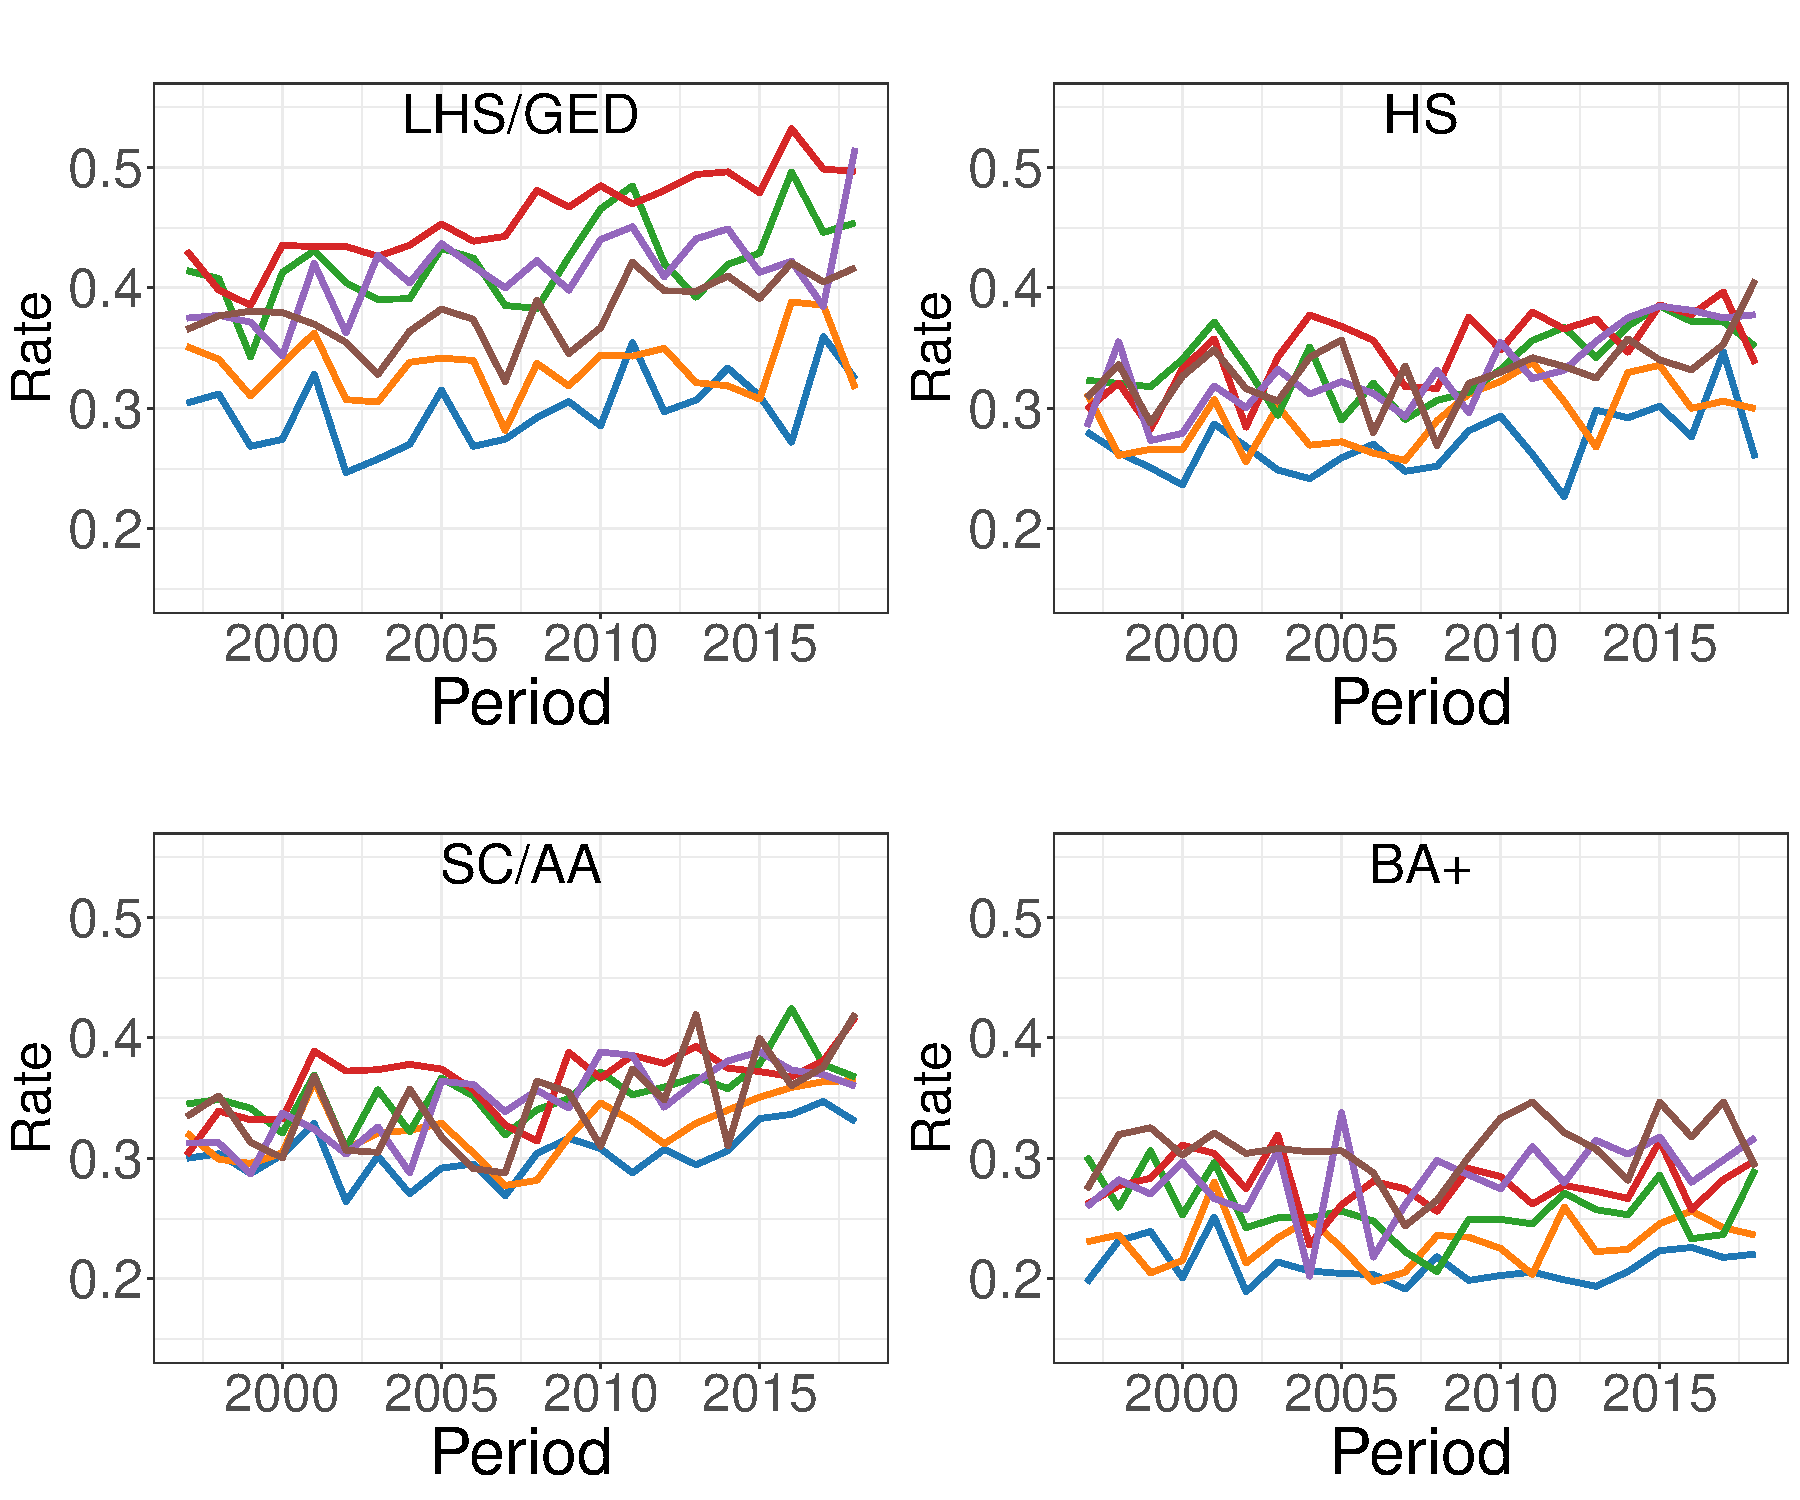
\includegraphics[width=1.6\linewidth]{Figures/rateplot_age_f.pdf}
    \end{minipage}%
    \begin{minipage}{.5\textwidth}
      \hfill
      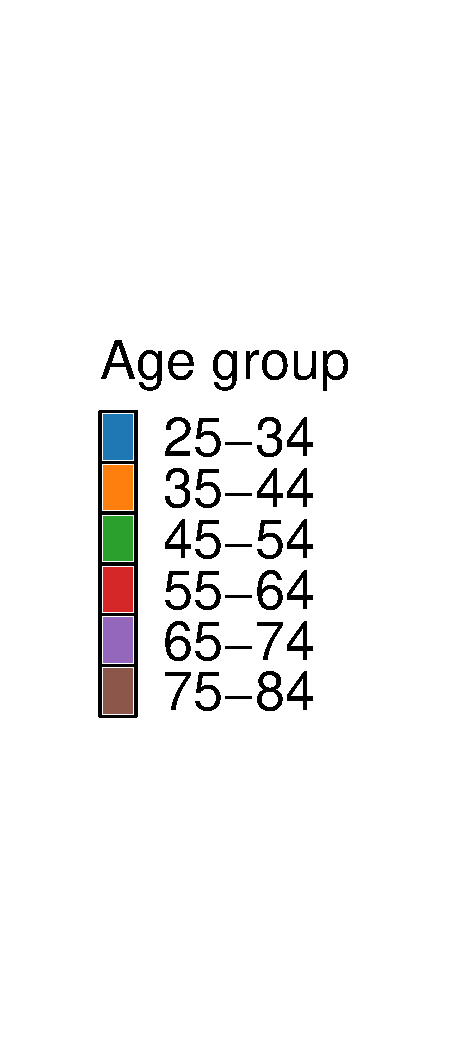
\includegraphics[width=0.4\linewidth]{Figures/rateplot_age_legend_f.pdf}
    \end{minipage}
    \caption{The proportion of female survey participants with back pain over periods, grouped into $6$ groups by age for each level of attained education.}
    \label{figure:explorative:rateplot_age_f}
\end{figure}

\begin{figure}[!ht]
    \centering
    \begin{minipage}{.5\textwidth}
      \centering
      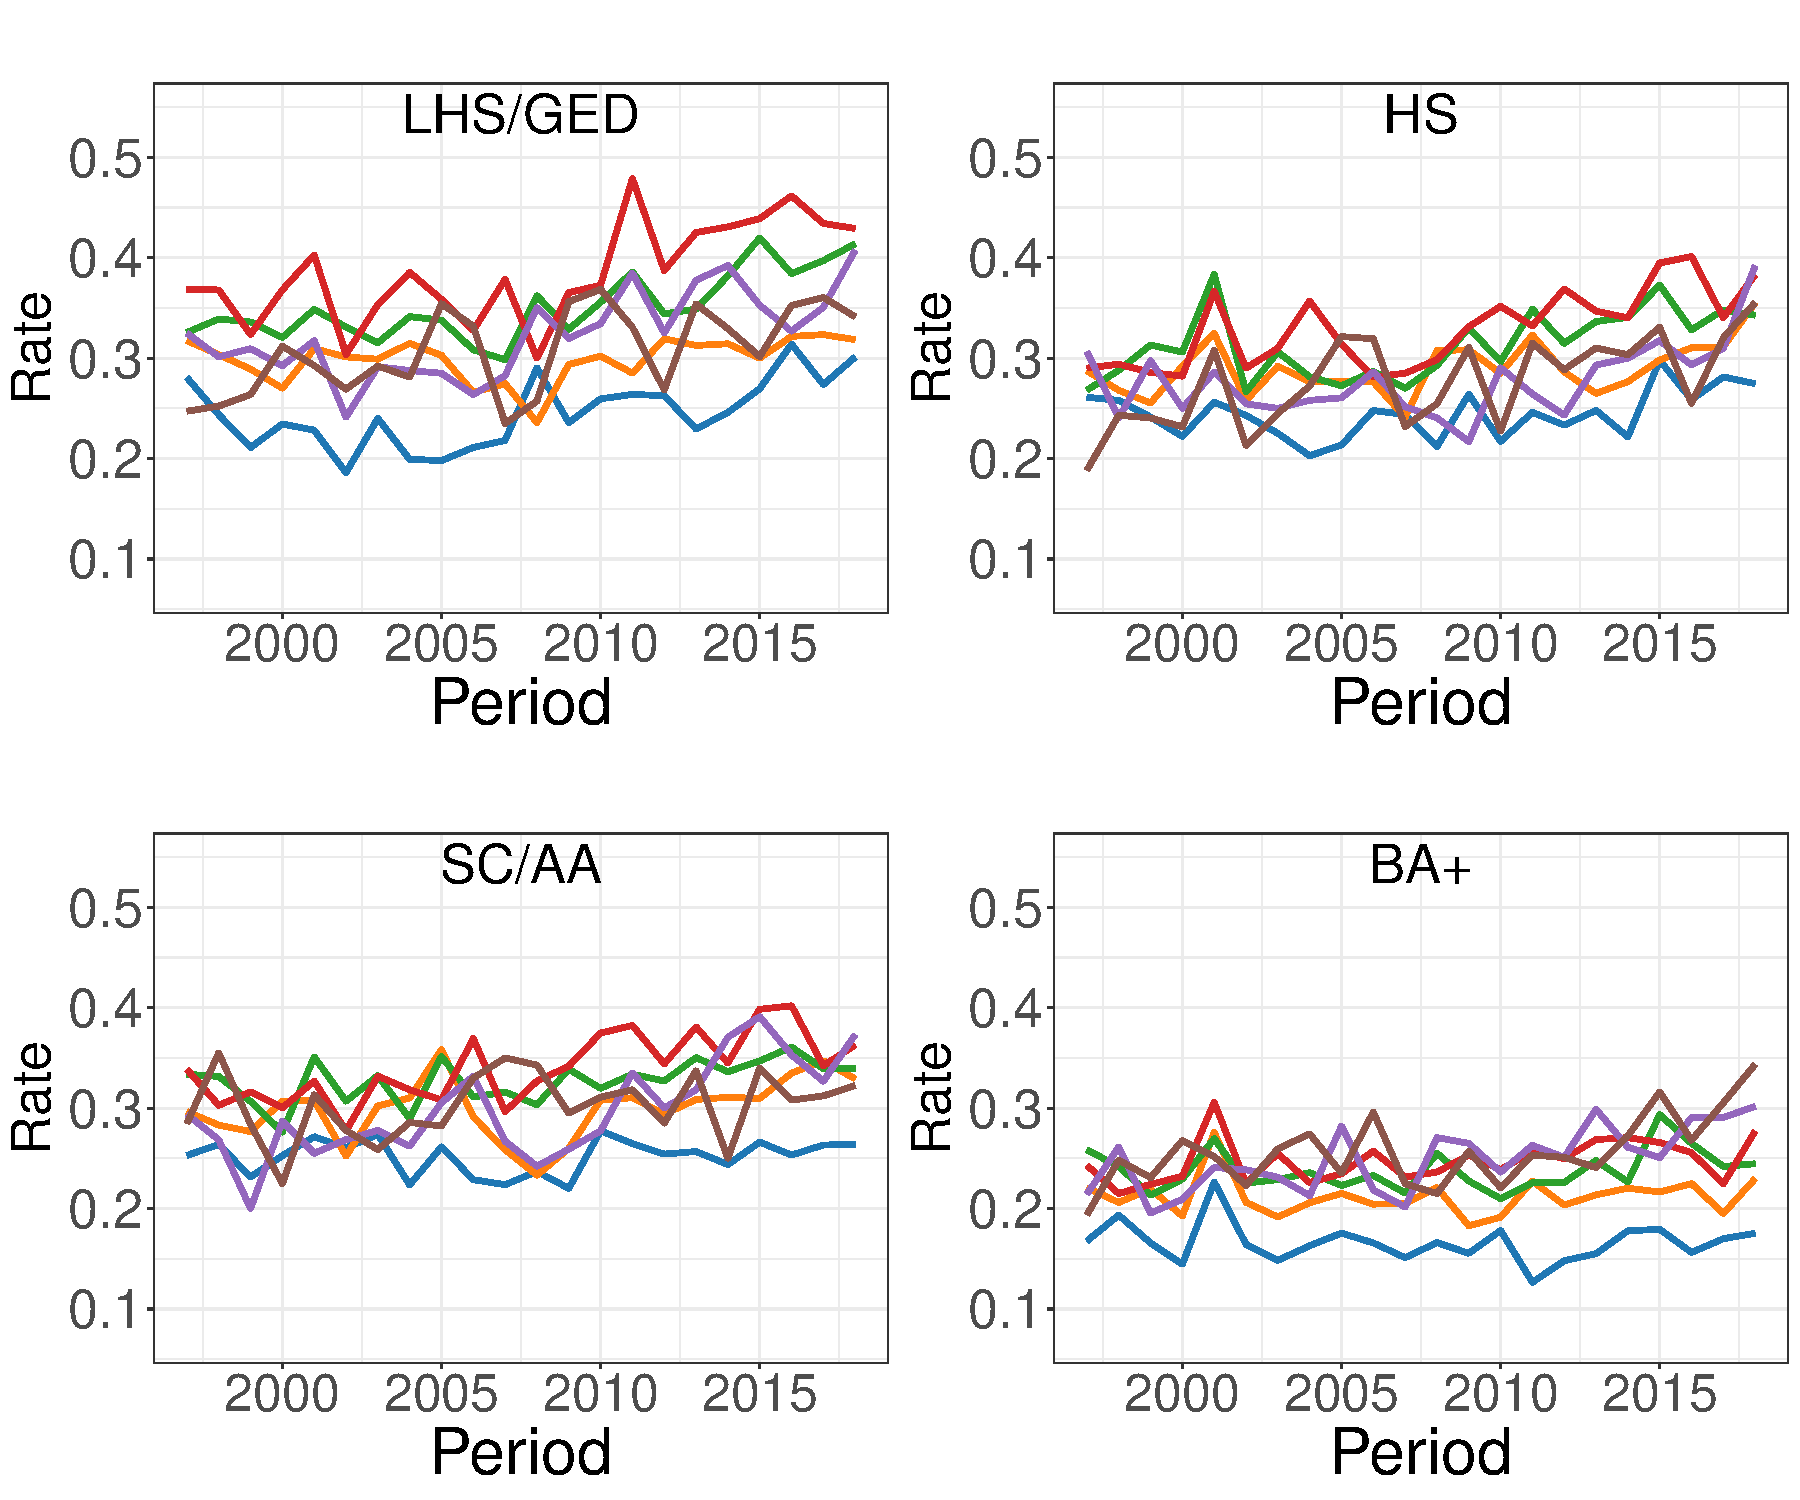
\includegraphics[width=1.6\linewidth]{Figures/rateplot_age_m.pdf}
    \end{minipage}%
    \begin{minipage}{.5\textwidth}
      \hfill
      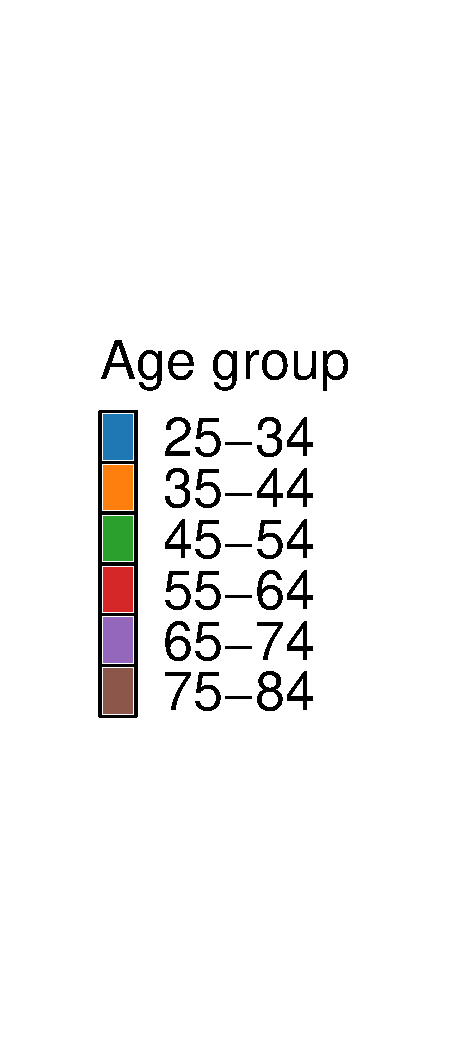
\includegraphics[width=0.4\linewidth]{Figures/rateplot_age_legend_m.pdf}
    \end{minipage}
    \caption{The proportion of male survey participants with back pain over periods, grouped into $6$ groups by age for each level of attained education.}
    \label{figure:explorative:rateplot_age_m}
\end{figure}

Figures \ref{figure:explorative:rateplot_cohort_f} and \ref{figure:explorative:rateplot_cohort_m} show the rate of back pain over the years of observation in survey participants grouped by generation (over several birth cohorts) for females and males, respectively. Generally, within all educational groups, we observe a larger rate of back pain in older generations and smaller rates for more recent generations. For the newest generation, the rate is particularly low among participants with the lowest level of attained education. For the oldest generation, however, more variability is observed, making it difficult to compare with the others. This variability is somewhat expected, as the sample size from the oldest generation is quite small, and the low rate of back pain could be due to the exceptionally good health of the survivors of this generation. This is reminiscent of an effect well known in demography, known as selective mortality \citep{beckett2000converging, house1990age, lynch2003cohort}. As with the effects grouped by age, the rate of back pain in all levels of education appears to be either constant or somewhat increasing. 


\begin{figure}[!ht]
    \centering
    \begin{minipage}{.5\textwidth}
      \centering
      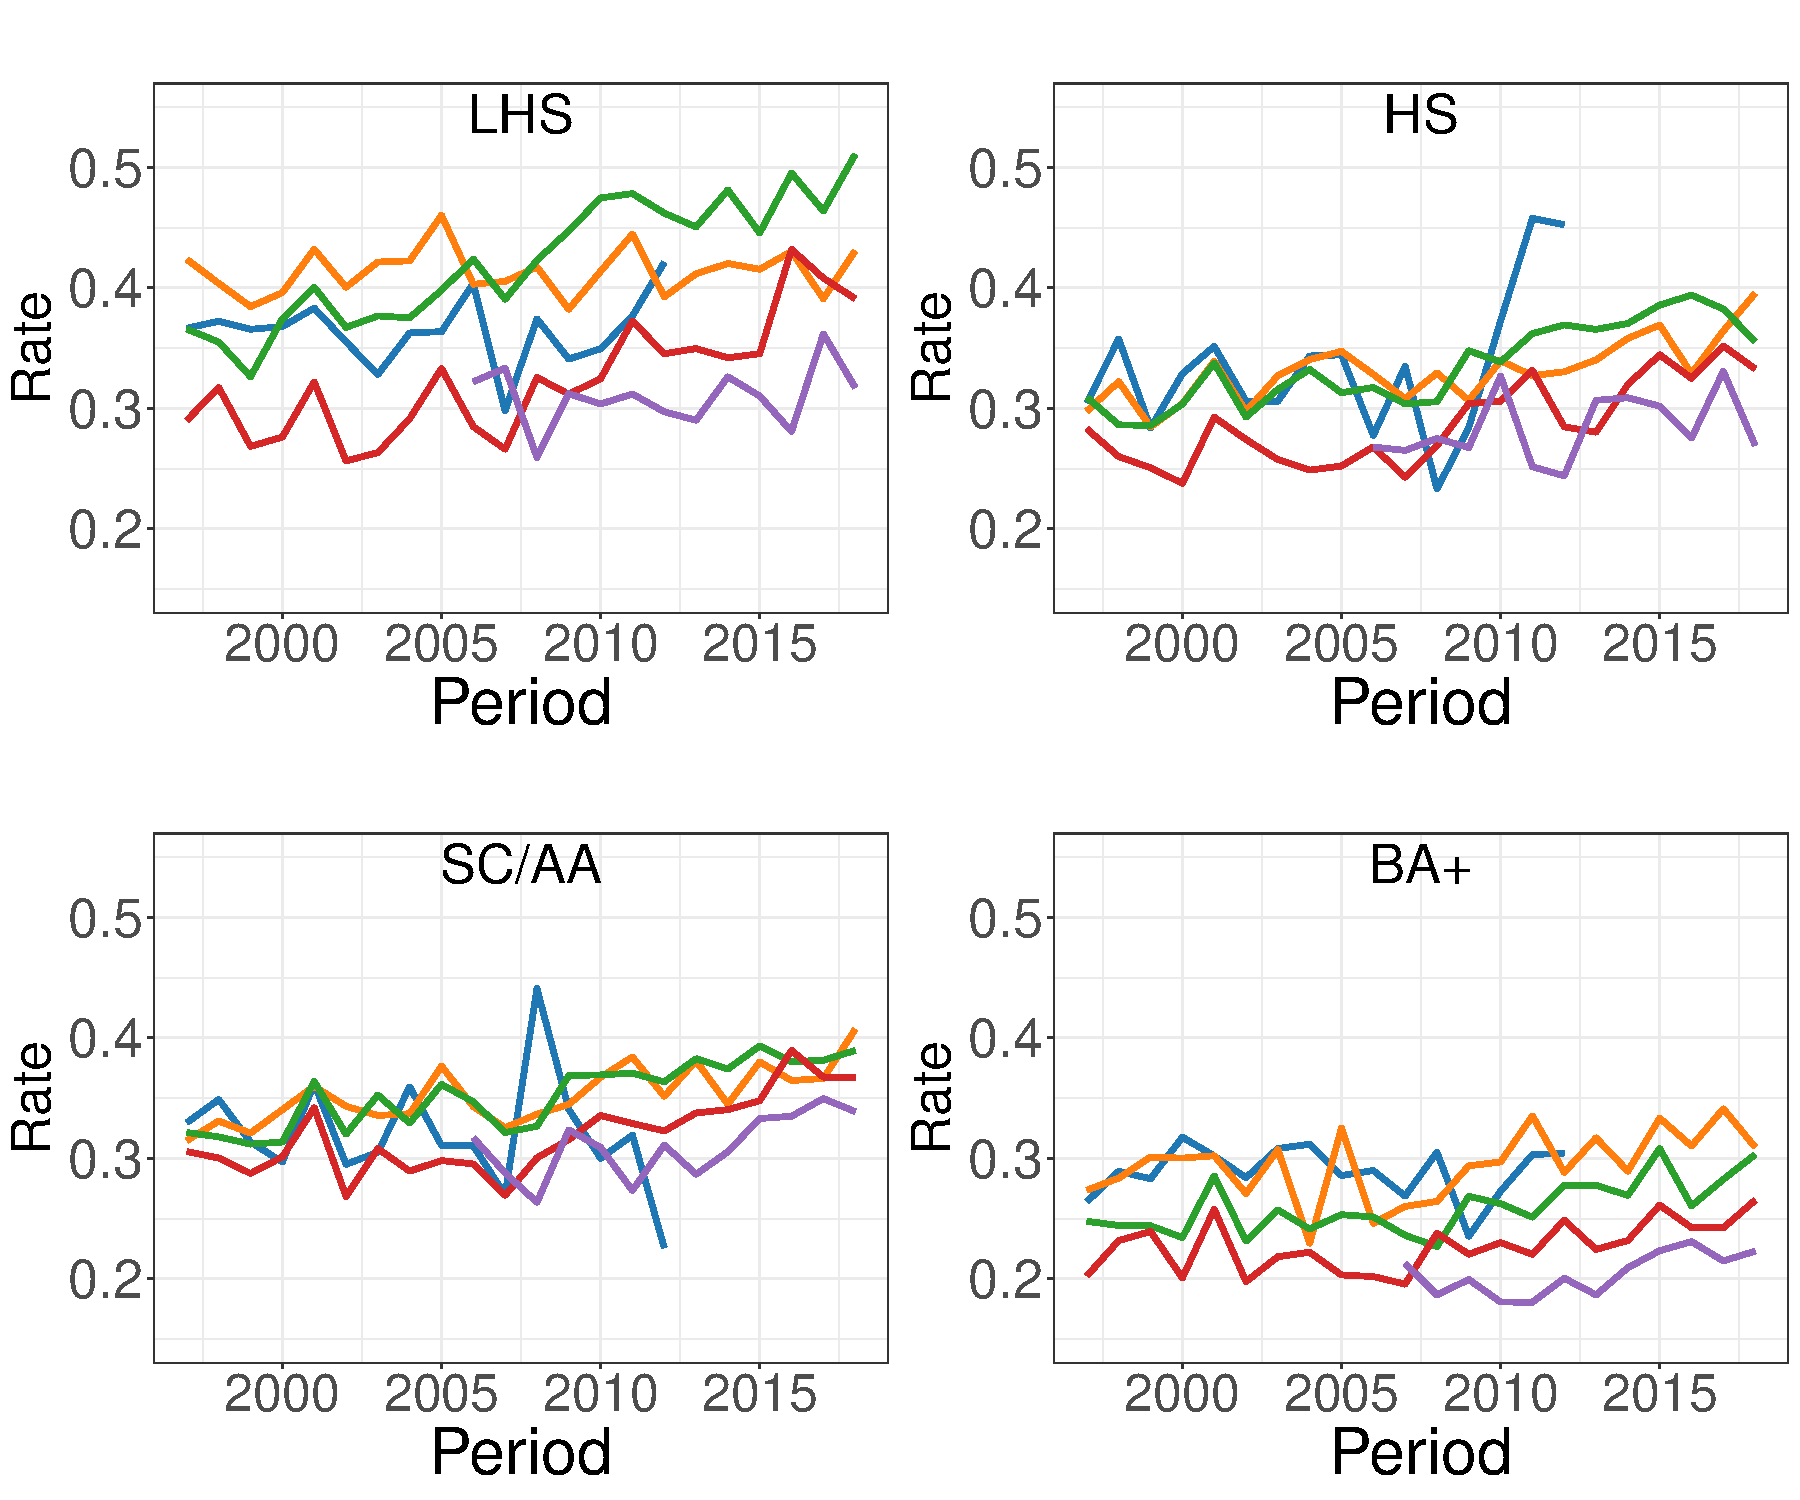
\includegraphics[width=1.6\linewidth]{Figures/rateplot_cohort_f.pdf}
    \end{minipage}%
    \begin{minipage}{.5\textwidth}
      \hfill
      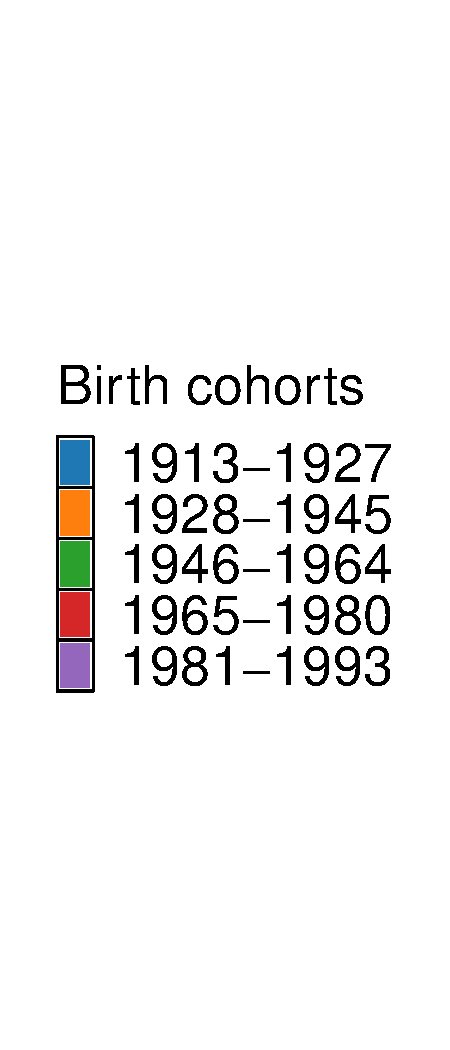
\includegraphics[width=0.4\linewidth]{Figures/rateplot_cohort_legend_f.pdf}
    \end{minipage}
    \caption{The proportion of female survey participants with back pain over cohorts, grouped into $6$ groups by age for each level of attained education.}
    \label{figure:explorative:rateplot_cohort_f}
\end{figure}

\begin{figure}[!ht]
    \centering
    \begin{minipage}{.5\textwidth}
      \centering
      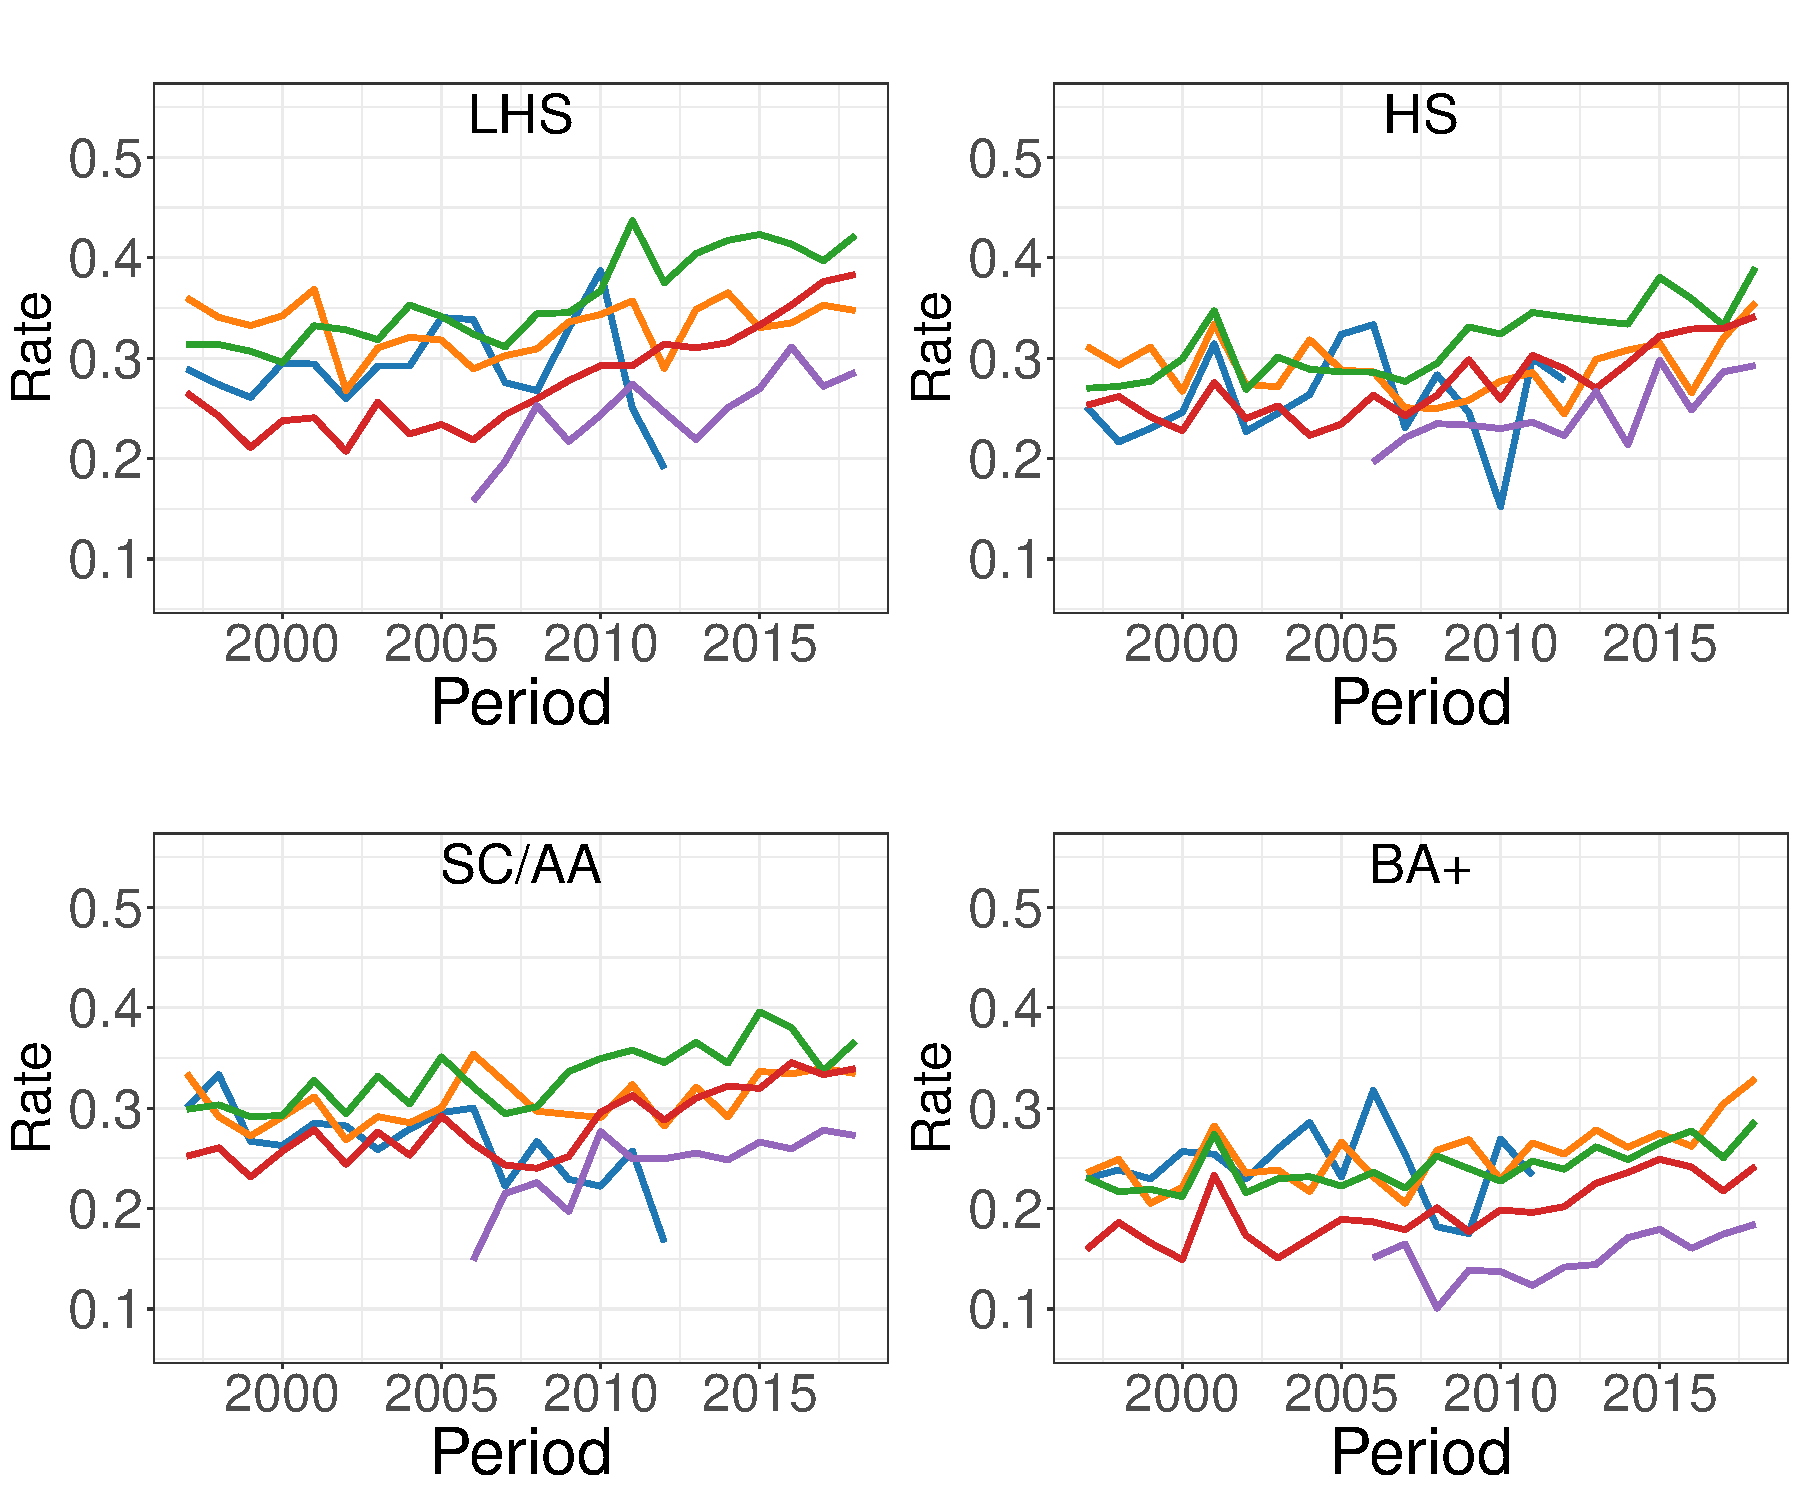
\includegraphics[width=1.6\linewidth]{Figures/rateplot_cohort_m.pdf}
    \end{minipage}%
    \begin{minipage}{.5\textwidth}
      \hfill
      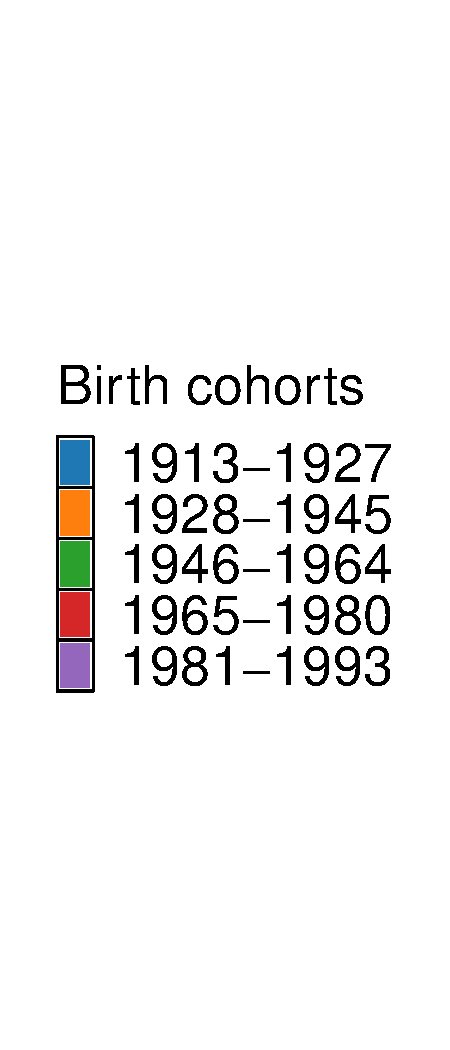
\includegraphics[width=0.4\linewidth]{Figures/rateplot_cohort_legend_m.pdf}
    \end{minipage}
    \caption{The proportion of male survey participants with back pain over cohorts, grouped into $6$ groups by age for each level of attained education.}
    \label{figure:explorative:rateplot_cohort_m}
\end{figure}

By this simple exploratory analysis, we may theorize on what to expect from the analysis by MAPC models. Firstly, as the rate of back pain stratified by attained education remains almost constant over periods in several age groups and cohorts, we do not expect the period as a temporal scale to be of large significance in explaining the observed temporal variability. Moreover, due to the observable differences in rate based on age groups for all levels of education, it is expected that age as a temporal scale will be of great significance. Since these differences in rate based on age groups were particularly pronounced for LHS/GED level of attained education, we expect this to be reflected in our models. The same is said for cohort, as similar observations were made over this temporal scale and the differences are more pronounced for the LHS/GED level. In addition, since it is clear that participants with BA+ level of attained education generally had better health outcomes and had larger sample sizes over all temporal indices, it would be sensible to pick this level of attained education as our baseline level of attained education for later inference across levels of attained education.











